\documentclass[times, utf8, seminar]{fit}

%\batchmode
%\usepackage{booktabs}
\usepackage{listings}
\usepackage{longtable}
\usepackage{xcolor}
\usepackage{float}
\usepackage{enumitem}
\usepackage{hyperref}
\usepackage{enumerate}
\usepackage{graphicx}
\usepackage{etoolbox}

\begin{document}

\title{Projekat: Unapređenje informacionog sistema na primjeru jedne kompanije}

\author{Ernad Husremović}
\brindex{DL 2792}
\verzija {1.0.1}

\mentor{prof.dr Murat Prašo}

\maketitle

\tableofcontents

\listoftables
\listoffigures

% abstract begin
\begin{sazetak}

Ovaj rad prikazuje projekat unapređenja poslovnog informacionog sistema (IS) u kompaniji koja trenutno posjeduje IS baziran na nelegalnom software-u. 
Novi IS je baziran na software-u otvorenog koda \engl{open source software, OSS}.
Pored standardnih OSS aplikacija, za komponentu poslovnog rješenja korišteno je "F18 knowhowERP" programsko rješenje kompanije "bring.out" doo Sarajevo. "F18" je multiplatformski OSS software.
U radu su detaljno objašnjenje prednosti i nedocstaci uvođenja takvog IS-a.
Izvršena je analiza svih bitnih aspekata realizacije takvog projekta, kako tehničkih i tako i ekonomskih. 

\kljucnerijeci{projekat, software otvoreng koda, OSS, multiplatformski sofver, poslovne aplikacije, F18, ERP, bring.out, informacioni sistem, IS}
\end{sazetak}

\engtitle{Project: Improvement of the information system - Case study}
\begin{abstract}

This report presents the details of the project which aimed to improve business business information system (IS) in a company which currently owns an IS based on an illegal software. The new IS was designed as an open platform. Appart of the standard applications tis project also incorporated ERP (Enterprise resource planning) software component "F18 knowhowERP", produced by "bring.out" doo Sarajevo. "F18" is an OSS multiplatform software. This report explains what OSS represents for the user with all advantages and risks. The detailed analysis conaining all relevant aspects of the project is also presented.

\keywords{project, open source software, OSS, multiplatform software, business application, F18, ERP, bring.out, information system, IS, illegal software}
\end{abstract}

% abstract end

\chapter{Uvod}

\section{Uticaj akcije legalizacije na promjene na IT tržištu BiH}

Akcije državnih inspekcijskih organa na suzbijanju nelegalnog software-a (nadalje legalizacija) sa početkom 2012 godine označila je početak krupnih promjena na tržištu informatičkih \engl{information technology, nadalje IT} rješenja u Bosni i Hercegovini. 
Većina poslovnih subjekata koja je proteklih godina koristila nelegalni software \engl{software} našla se u nezavidnoj situaciji.
Usljed visokih troškova legalizacije "Microsoft" sofware-a\footnote{familija "Microsoft Windows" OS-ova, uz svuda prisutni ali i redovno nelegalno instalirani "Microsoft Office" uredski paket}, pojavila se potražnja za software-om drugih proizvođača.  

\section{Open source software u BiH}

Preduzeće "bring.out"\footnote{\url{http://www.bring.out.ba/}} je dugi niz godina orjentisano na ponudu sistema baziranih na software-u otvorenog koda \engl{open source software, nadalje OSS}.
Potražnja za Linux/Ubuntu serverskim rješenjima \footnote{\url{http://linux.com}, \url{http://ubuntu.com}}) je postojala i prije legalizacije. Međutim, tek nakon legalizacije pojavila se potražnja za cjelovitim informatičkim IT rješenjima baziranim na OSS-u:
\begin{itemize}
  \item server operativni sistem (nadalje OS)
  \item desktop operativni sistem
  \item aplikativni software
  \begin{itemize}
    \item opći software za uredske potrebe
    \item poslovni software za podršku tekućim operacijama kompanije \engl{Enterprise Resource Planning, nadalje ERP}
  \end{itemize}
\end{itemize}

\subsection{Ubuntu Linux}
"Ubuntu Linux" distribucija je radi svoje jednostavnosti i kvaliteta postao iznimno popularan desktop OS. Za razliku od "Windows" operativnih sistema, "Ubuntu" desktop sistem sadrži kompletan set aplikacija za svakodnevne potrebe:
\begin{itemize}
  \item LibreOffice uredski paket za pravljenje tekstualnih i tabelarnih dokumenata, prezentacija i crteža\footnote{U funkcionalnom smislu sličan "Microsoft office" setu aplikacija. Može obrađivati većinu "Microsoft office" dokumenata}
  \item "Inkscape", program za vektorsku grafiku \cite{inkscape}
  \item "GIMP", program za bitmapiranu grafiku
  \item "Evince", preglednik PDF dokumenata
  \item "Firefox", "Chromium" internet pretraživači
  \item "OpenProj", program za izradu i praćenje projekata\footnote{U funkcionalnom smislu sličan "Microsoft project" aplikaciji}
\end{itemize}  

\subsection{Razlike između otvorenog i zatvorenog software-a} 

Lista iz predhodne sekcije predstavlja djelimičnu listu aplikacija dostupnih za "Ubuntu". Međutim, i to je dovoljno da se uoči bitna razlika između "Windows"-a i "Ubuntu"-a:
\begin{enumerate}
  \item Uz "Windows" početni paket se isporučuje samo operativni sistem, dok "Ubuntu" (kao i ostale Linux distribucije) isporučuju kompletan sistem koji korisnik može odmah početi koristiti.
  \item Razvoj "open source" software-a je suštinski drugačiji u odnosu na razvoj zatvorenog sofvera \cite{bazaar}. Kod zatvorenog software-a sve ključne razvojne aktivnosti i sudbina software-a nalaze se u rukama jednog proizvođača. Kod OSS-a postoji velika uključenost zajednice korisnika \engl{community}, što omogućava da se sve komponente software-a razvijaju u skladu sa potrebama i zahtjevima korisnika. 
  \item U ranom stadiju razvoja OSS software je manjkao sa kvalitetnom dokumentacijom. Sada to nije slučaj. Korisnicima je na raspolaganju velika količina dokumentacije koja se takođe razvija na principima otvorenosti. Tako korisik "Ubuntu" sistema na raspolaganju ima odličnu dokumentaciju za serverske \cite{ubuntudesktop} i desktop \cite{ubuntuserver} sistem.
  \item Zahvaljujući otvorenosti, lokalizacija programa i korisničke dokumentacije (prevod i prilagodbe za lokalno tržipte) za OSS nije vođena samo komercijalnim motivima. S druge strane lokalizacija "Microsoft" proizvoda ovisi isključivo o komercijalnim faktorima. Zato je stepen lokalizacije "Microsoft" software-a na malim tržištima kakvo je naše minimalan.   
\end{enumerate}

U mnogim zemljama postoje jake zajednice korisnika koje lokalizaciju "open source" software-a vrše na bazi volonterizma. Kako se radi o projektima od velikog javnog značaja, te zajednice su često finansirane od strane države. 
Svijetli primjeri država u regionu u kojima postoje jake zajednice FOSS \engl{Free and open source software} \& OSS  korisnika su Makedonija i Slovenija.
Na žalost, Bosna i Hercegovina, kao i u većini stvari, na tom planu zaostaje. 

\subsection{"F18 knowhowERP" software}
Pored standardnih komponentni "Ubuntu" OS-a, za ERP software je korišten "F18" knowhowERP software.

"F18" knowhowERP\footnote{\url{http://redmine.bring.out.ba/projects/f18}} je multiplatformsko "open source" ERP rješenje, proizvod firme "bring.out". Predhodnik "F18" je programsko rješenje "FMK" koje se na lokalnom tržištu koristi od 1994 godine. "F18" je software pravljen od Bosanaca za BiH tržište. "F18" je u cjelosti domaći proizvod.

Na osnovu svega što je do sada izloženo, bosanskom klijentu je moguće ponuditi cjelovito OSS IT rješenje.  Ovaj projekat će obuhvatiti instalaciju jednog takvog sistema kod klijenta.

\chapter{Analiza}

\section{Profil korisnika projekta}
Korisnik je mala kompanija koja se bavi trgovinom. Sa stanovišta IT-a kompanija se sastoji od:
\begin{itemize}
  \item maloprodajna mreža od 5 prodavnica
  \item centrala kompanije sa knjigovodstvom, 4 radne stanice
  \item 1 server baze podataka 
\end{itemize}
\pagebreak
\section{Analiza problema}
Glavni razlog zbog kojeg se klijent obratio bila je potreba da uvede legalni software. Analiza postojećeg stana urađena je uz pomoć modela piramide problema (\cite{prasopro}). Model piramide problema omogućava hijerarhijski prikaz problema od općih ka konkretnim: 

\begin{figure}[H]
\centering
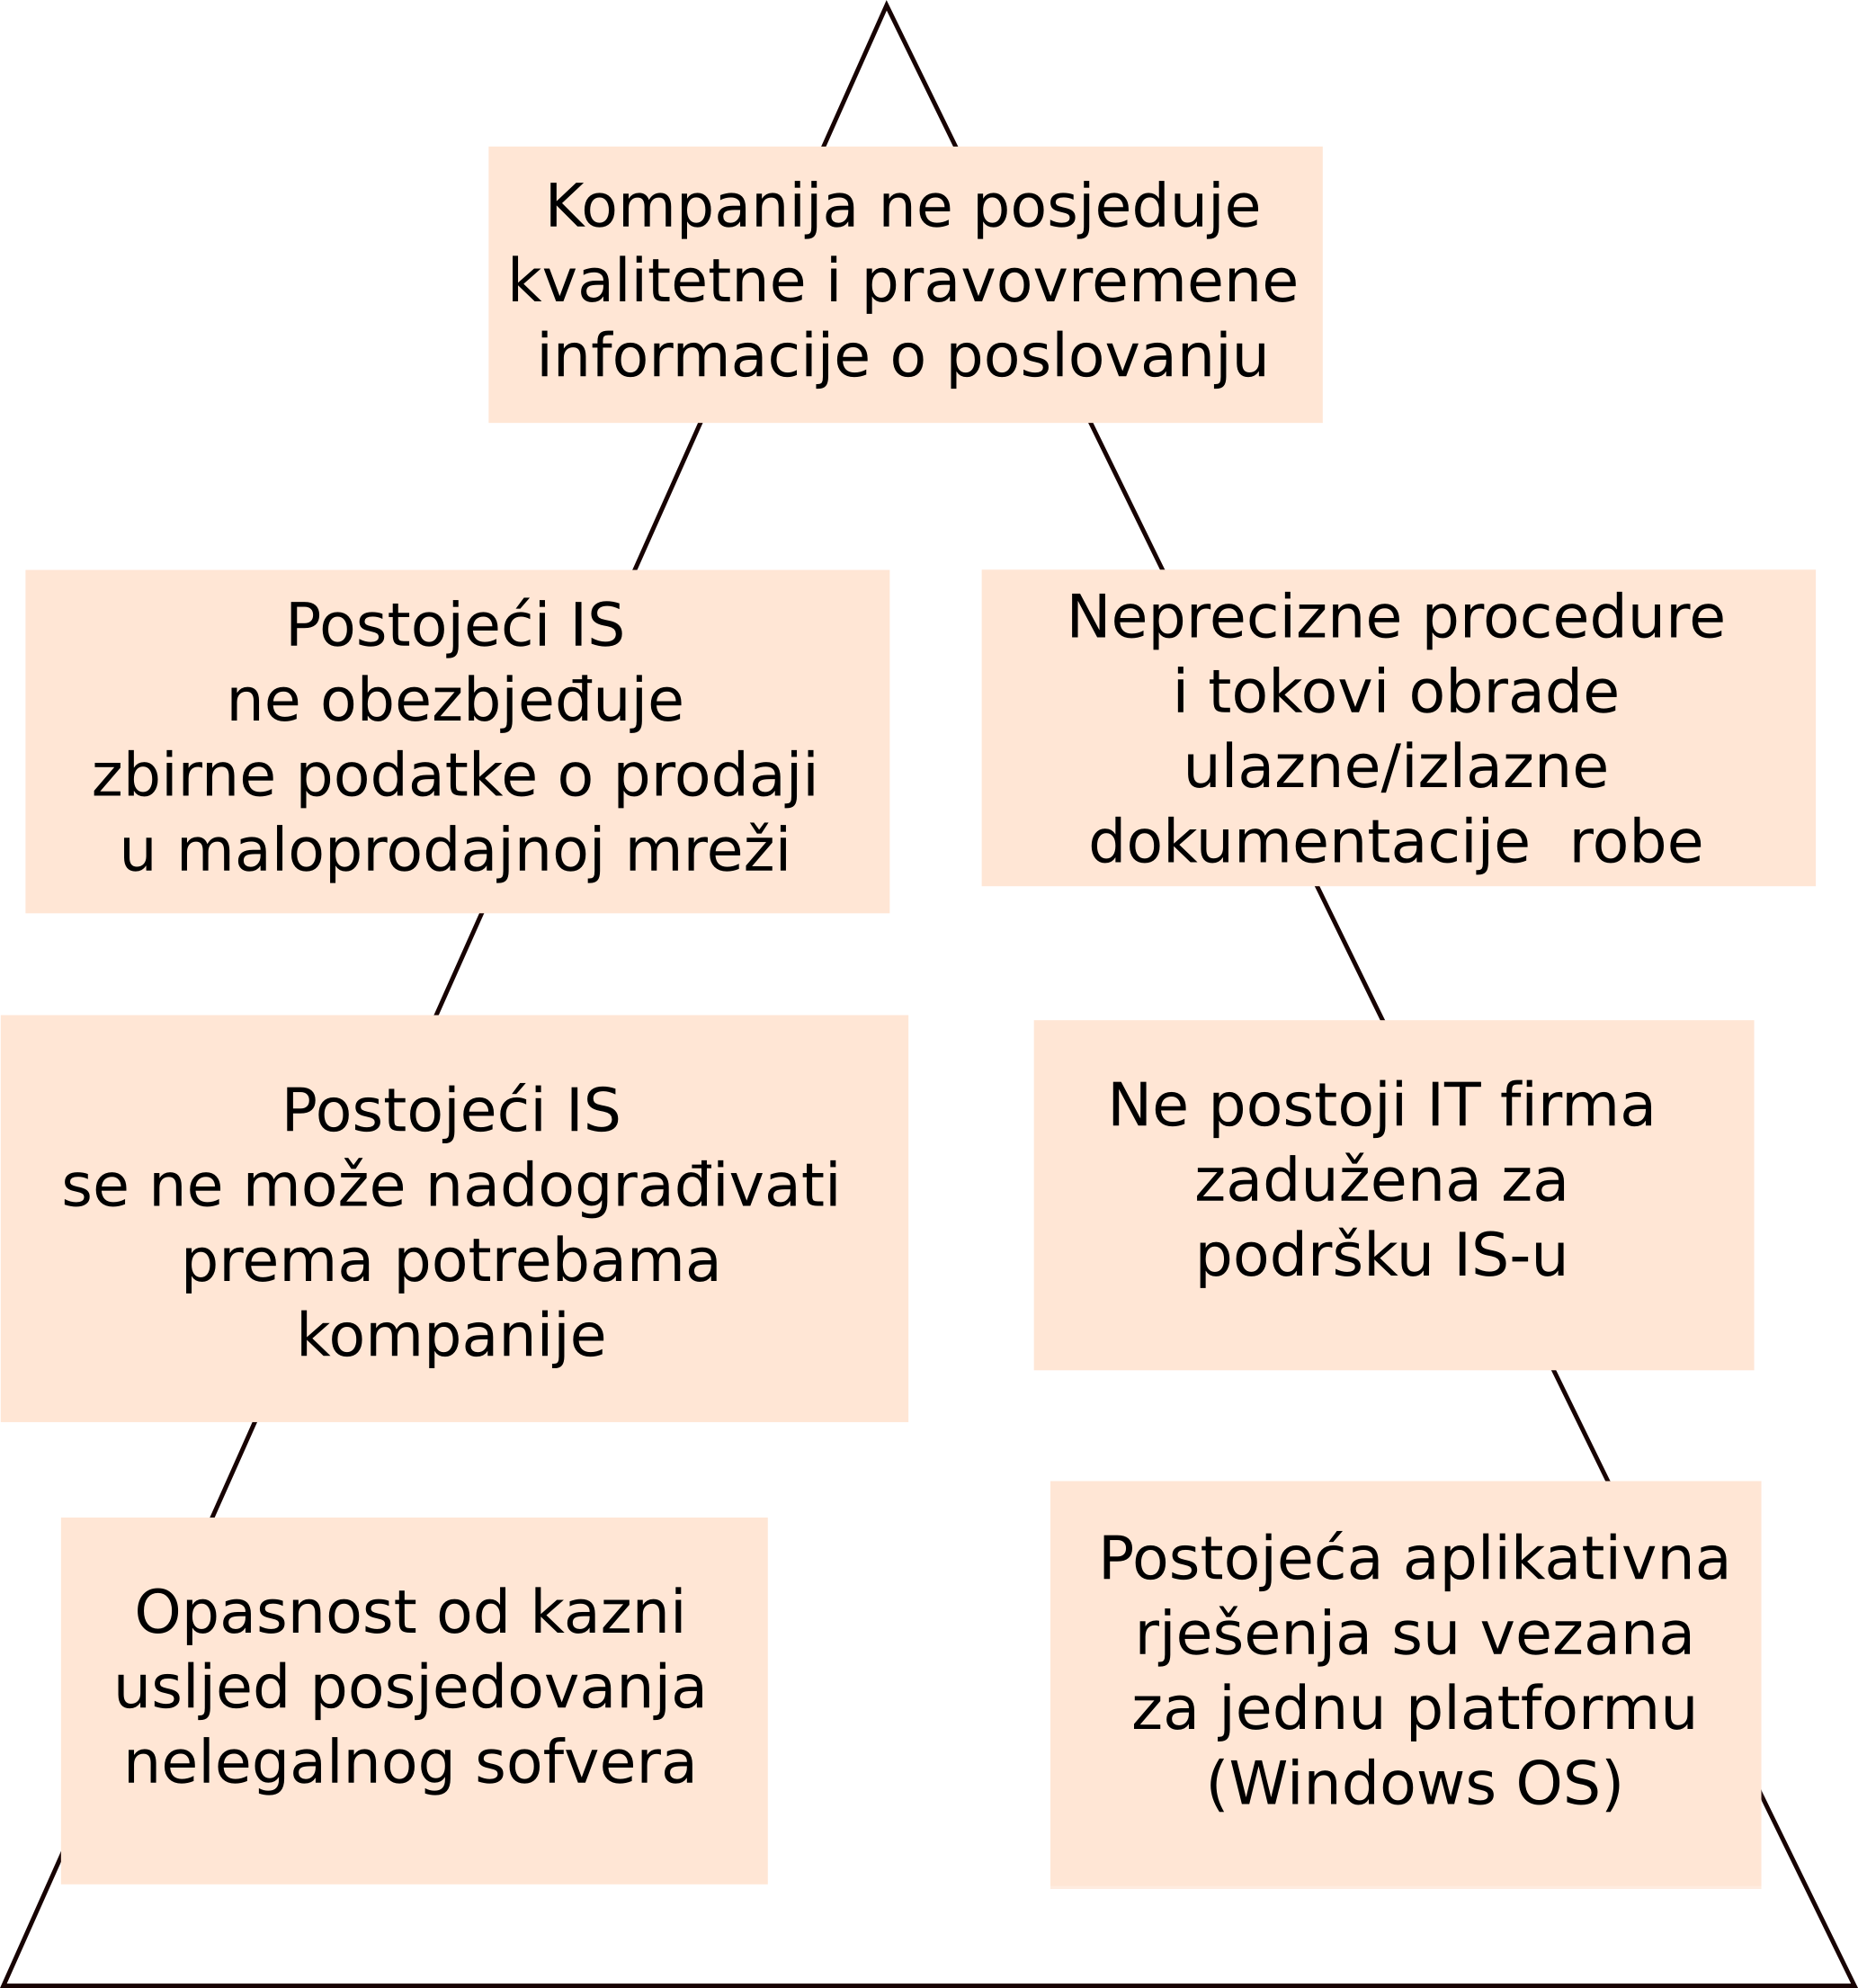
\includegraphics[width=10cm]{img/piramida_problema.png}
\caption{Piramida problema}
%\caption{bla bla (\cite{web:eric})}
\end{figure}

\pagebreak
\section{Definisanje ciljeva projekta}
Na osnovu analize problema definisana je piramida ciljeva projekta: 

\begin{figure}[H]
\centering
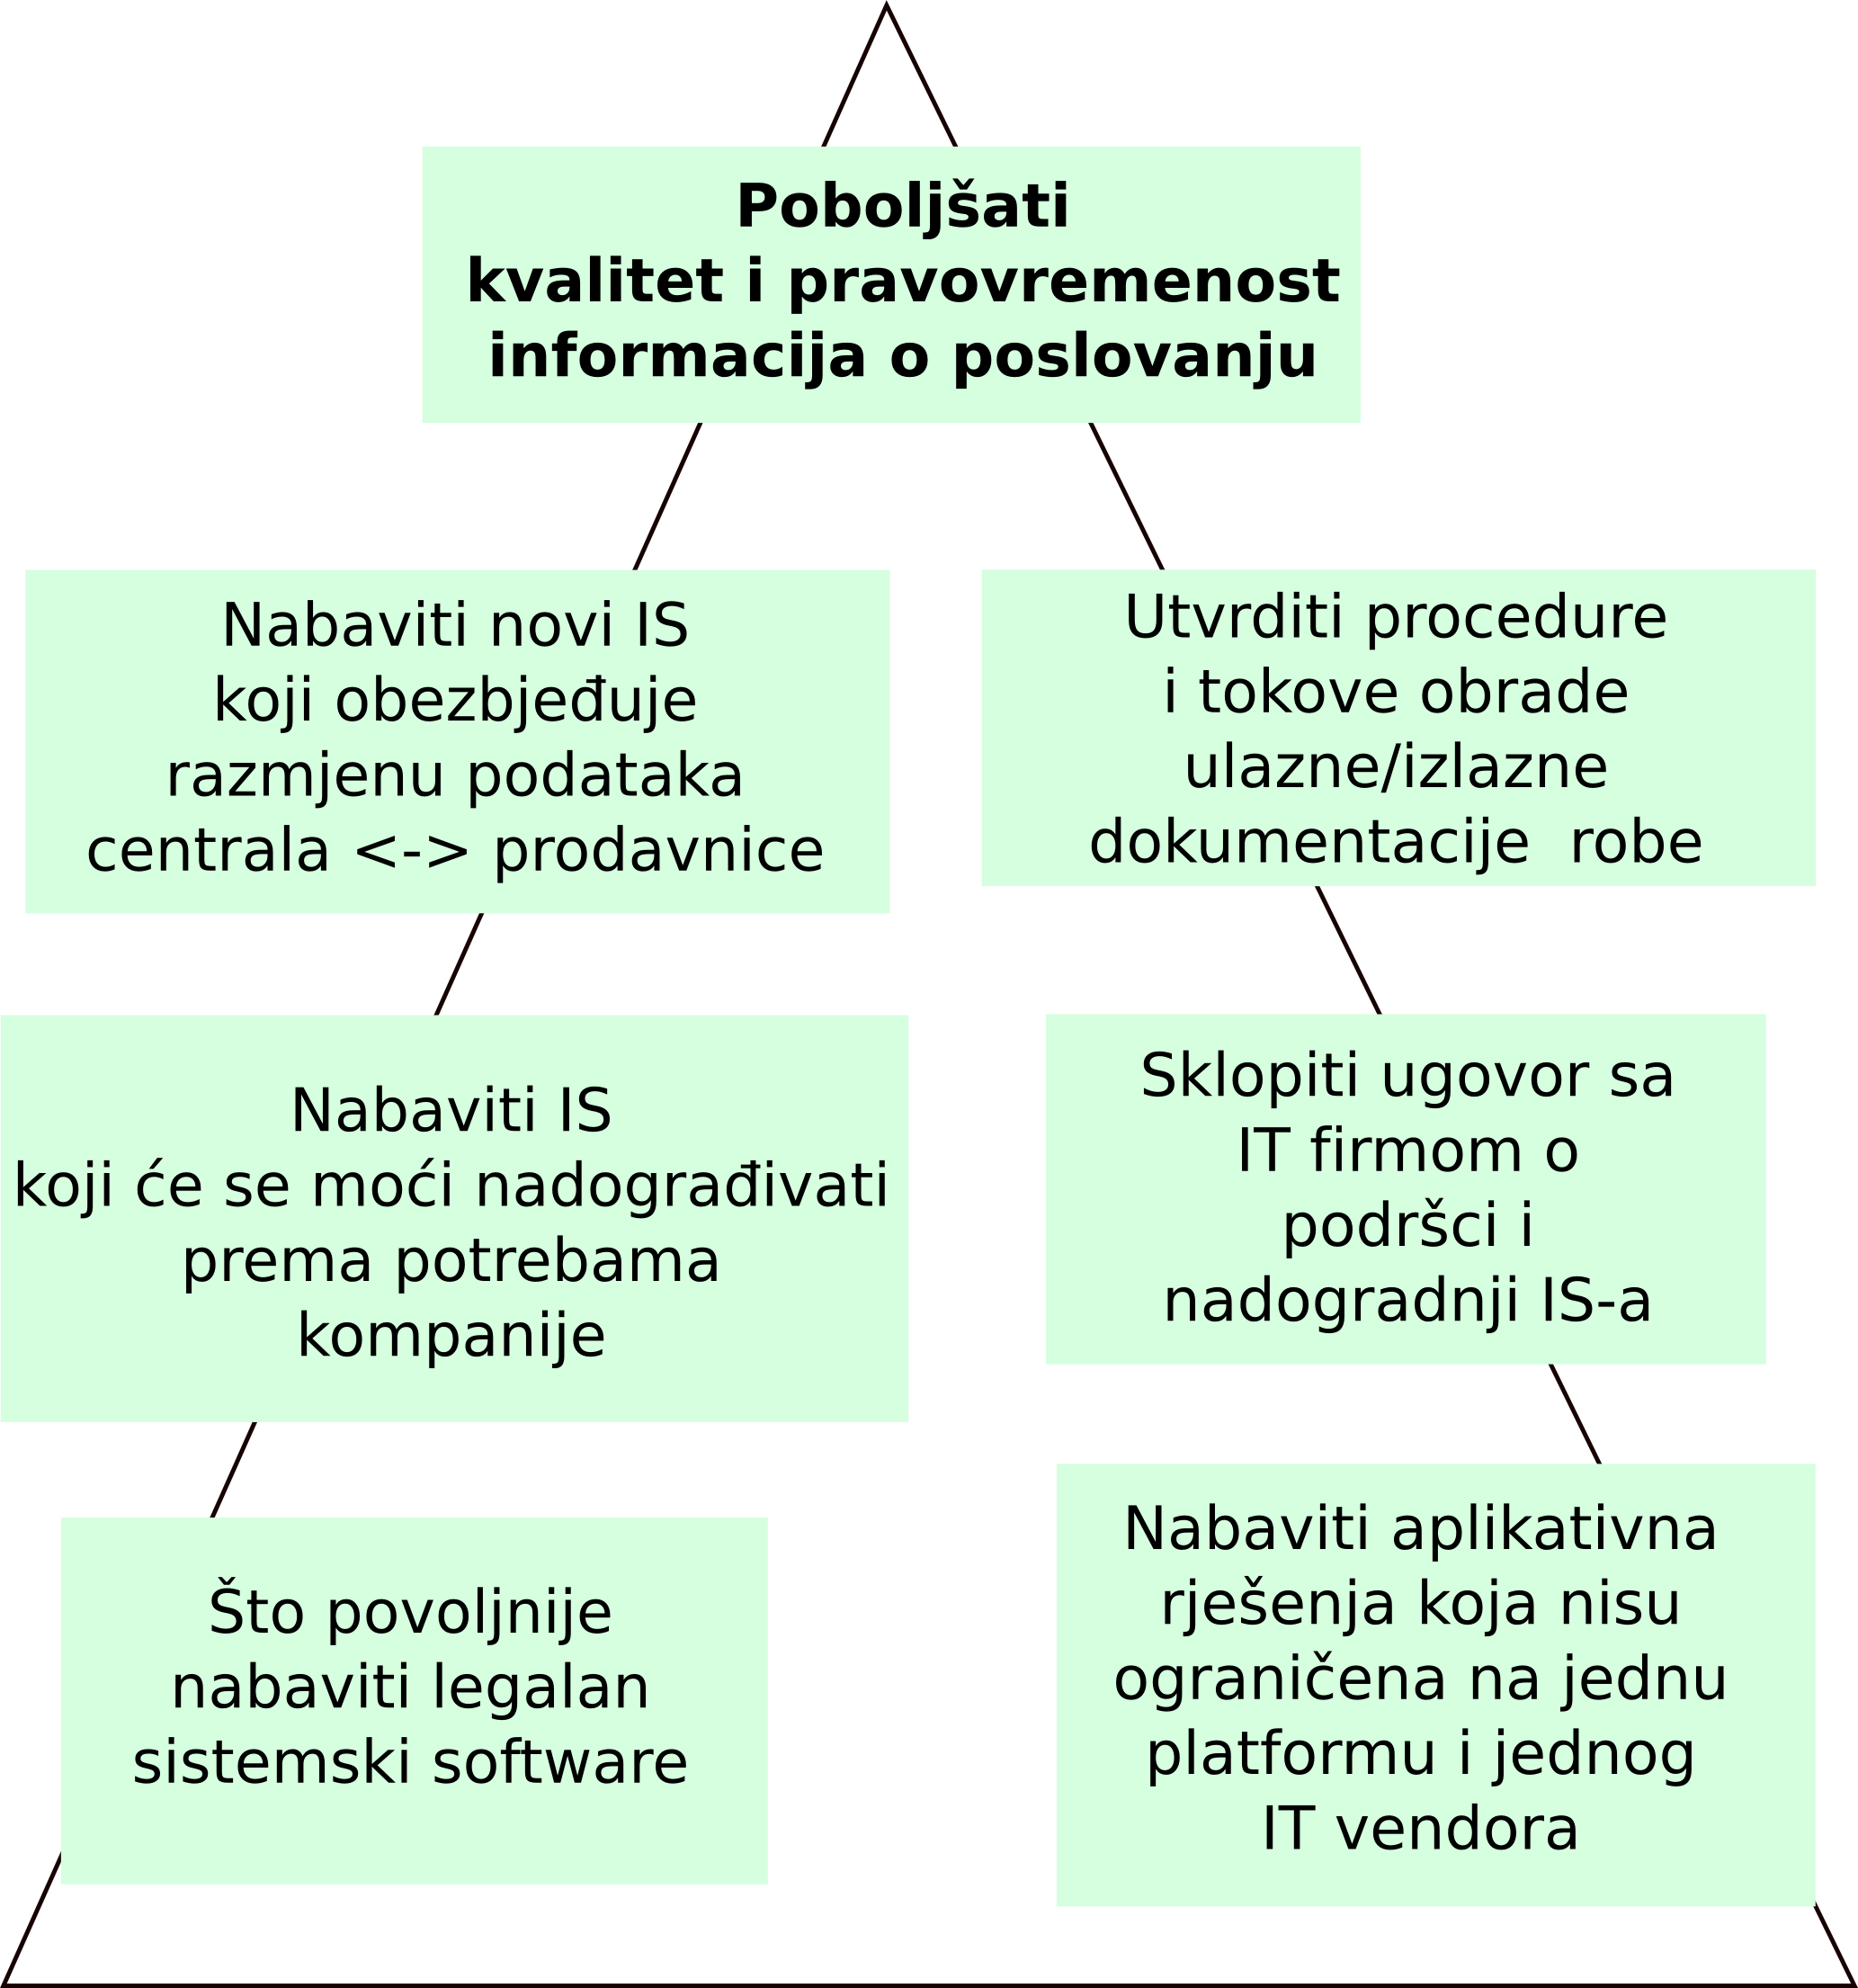
\includegraphics[width=10cm]{img/piramida_cilja.png}
\caption{Piramida cilja}
\end{figure}

Strateški cilj je poboljšati pravoremenost i kvalitet tekućih informacija o poslovanju kroz uvođenje novog IS-a. 

\section{Logički okvir projekta}
Na kraju analize dolazimo do ključnih odrednica projekta:
\begin{table}[h]
%\centering
\resizebox{15cm}{!} {
\begin{tabular}{ | r | l | }
\hline
Svrha projekta: & Unapređenje poslovanja kompanije obezbjeđenjem kvalitetnijih informacija o poslovanju \\ \hline
Cilj: & Uvođenje novog informacionog sistema \\ \hline
Ulazi projekta: & Postojeći informacioni sistem, postojeća organizacija poslovanja \\ \hline
Izlazi projekta: & Unapređeni informacioni sistem, unapređena organizacija poslovanja \\ \hline
\end{tabular}
}

\caption{Logički okvir projekta}
\end{table}

\chapter{Upravljanje projektom}

Upravljanje podrazumjeva uvid i praćenje svih bitnih aspekata projekta:
\begin{itemize}
  \item tehničkih
  \item vremenskih
  \item finansijskih
  \item identifikacija rizika
  \item planiranje ljudskih i materijalnih resursa
\end{itemize}

\section{Tehnički aspekti}

Komponente za realizaciju IS-a su multiplatformski i "open source" sofware:
\begin{itemize}
  \item Desktop OS: Ubuntu Linux 12.04 32bit
  \item Server OS: Ubuntu Linux 12.04 64bit
  \item Uredski software: LibreOffice 3.5
  \item Sofware za podršku poslovanju: knowhow ERP F18
  \item Baza podataka: PostgreSQL 9.1
\end{itemize}

Postojeći hardware klijenta je dobrih karakteristika, tako da će biti u potpunosti iskorišten.
\pagebreak
\section{Vremenski aspekti}

Dinamika realizacije projekta je utvrđena tokom preliminarnih razgovora sa klijentom. Kao okvirno vrijeme dogovoren je 1 mjesec za realizaciju uz dodatnih 2-3 mjeseca označenih kao period stabilizacije sistema. 

Napravljeni dinamički plan je u skladu sa ranijim dogovorom.

\begin{table}[!h]
\centering
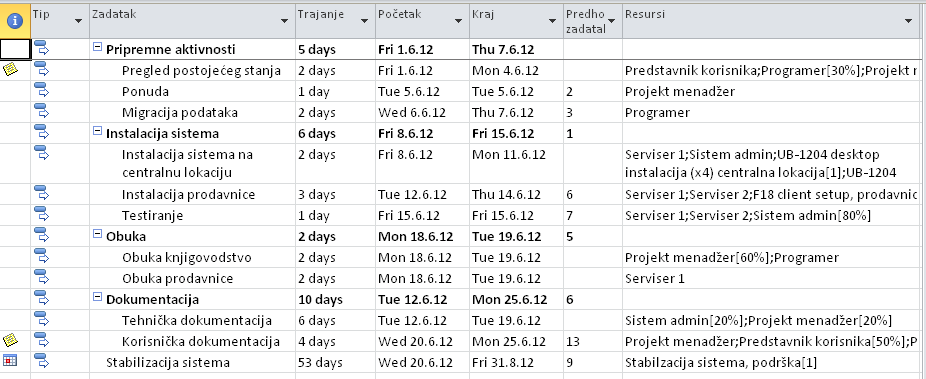
\includegraphics[width=15.5cm]{img/dinamika_sheet.png}
\caption{Tabelarni pregled projektnih zadataka}
\end{table}

\begin{figure}[!h]
\centering
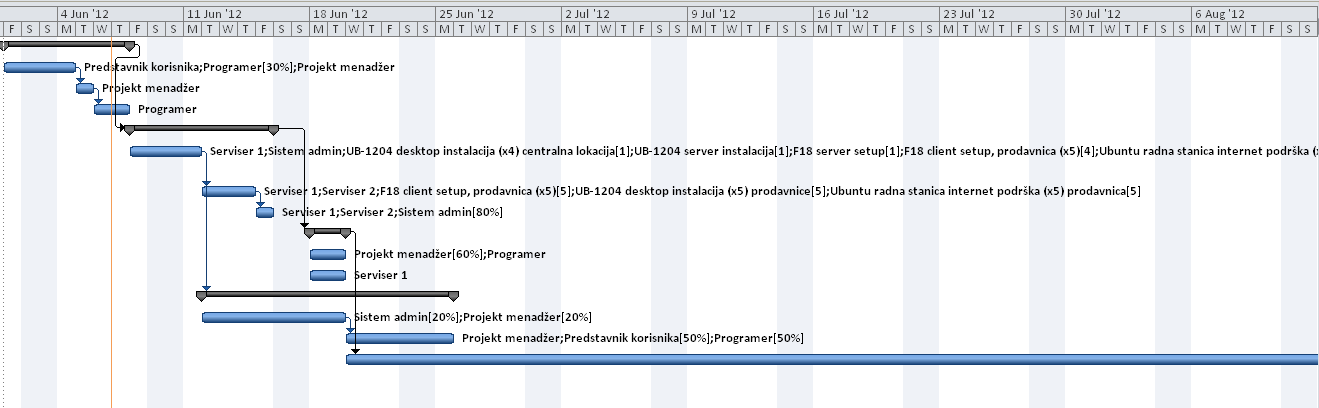
\includegraphics[width=15.5cm]{img/dinamika_gant.png}
\caption{Gantogram projekta}
\end{figure}

Vrijeme realizacije je \textbf{3 mjeseca}, period realizacije \textbf{01.06.2012 - 31.08.2012}.
%rizici
\section{Identifikacija rizika}
Identifikacijom i kvantifikacijom rizika napravljena je tabela rizika:
\begin{table}[!h]
\centering
\begin{tabular}{ |p{1.5cm}|p{4cm}|p{7.5cm}|p{1.5cm}| }
\hline
Oznaka & Rizik & Opis & Prioritet  \\ \hline\hline
R1 & Promjena navika kod korisnika & Novi IS pretpostavlja potpunu zamjenu software-a: od desktopa do ERP rješenja & Visok \\ \hline
R2 & bring.out je jedini OSS IT vendor na bosanskom tržištu & Iako su tehnologije koje se implementiraju otvorene, na BH tržištu ne postoje drugi vendori koji nude slična rješenja & Visok \\ \hline
R3 & Onemogućen pristup aplikacijama državnih institucija & IT rješenja državnih institucija u većini pretpostavljaju korištenje Windows OS-a & Visok \\ \hline
R4 & Ponuđeno ERP rješenje neće zadovoljiti potrebe klijenta & Opasnost da će klijent F18 knowhow ERP percipirati kao neadekvatno ERP rješenje & Srednji \\ \hline
R5 & Neredovno finansiranje projekta & Klijent neće moći obezbjediti redovno finansiranje projekta iz tekućih izvora & Srednji \\ \hline
\end{tabular}
\caption{Lista rizika po prioritetima}
\end{table}

\subsection{Strategija odgovora na pojedinačne rizike} 

U sljedećoj tabeli dajemo prikaz preventivnih i akcija kontrole za identificirane rizike:

\begin{table}[!h]
\centering
\begin{tabular}{|p{1.7cm}|p{13.2cm}|}
\hline
Oznaka & Preventivne i kontrolne akcije  \\ \hline\hline
R1 & Veću pažnju posvetiti obuci korisnika \\ \hline
R2 & Otvorenim pristupom klijentu pokazati klijenti da se odnosi da odnosi na relaciji otvoreni IT vendor <-> klijenta grade na partnerskog osnovi, a ne na bazi monopoliziranja znanja.\\ \hline
R3 & Aktivnim djelovanjem prema državnim institucijama obezbjediti da korisnici otvorenih sistema budu u istoj poziciji kao korisnici "Windows"-a\\ \hline 
R4 & IT vendor se treba aktivno uključiti u probleme i potrebe korisnika, pomoći mu da organizuje poslovanje u skladu sa  glavnim ciljevima IS-a, uzevši u obzir da je softver samo alat.\\ \hline
R5 & Zajedno sa klijentom definisati najprihvatljiviji finansijski plan za obje strane, a što je moguće upravo zahvaljujući činjenici da IT vendor nudi sopstvene proizvode i nije limitiran rokovima plaćanja prema svojim dobavljačima.\\ \hline
\end{tabular}
\caption{Prevencija i kontrola rizika}
\end{table}

%resursi
\section{Planiranje resursa}
\subsection{Materijalni resursi}
Pregled materijalnih resursa:
\begin{table}[h]
\centering
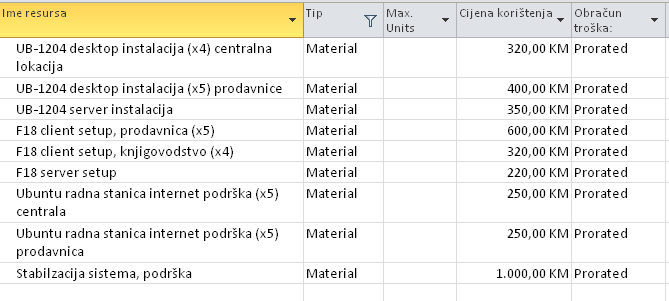
\includegraphics[width=15cm]{img/materijalni_resursi.png}
\caption{Pregled materijalnih resursa}
\end{table}

Treba naglasiti da se u slučaju "open source" sofvera ne radi o "klasičnim" materijanim resursima. Kod OSS-a prodaja licenci za korištenje kao troškovna stavka ne postoji. Klijent plaća instalaciju i podešenje sistema davaocu IT usluga \engl{IT vendor, IT provider}. S obzirom da su cijene tih usluga normirane, te usluge je najpogodnije u projektu izraziti kao materijalne resurse. 

Posebna ćemo prokomentarisati stavku "Stabilizacija sistema, podrška". Ova stavka predstavlja iznos ugovora o podršci u periodu stabilizacije sistema koji traje cca 2-3 mjeseca. U tom periodu se očekuju intenzivne aktivnosti servisnog i programerskog tima na rješavanju zahtjeva novog korisnika. Iako bi se moglo reći da ova stavka pripada periodu eksplotacije projekta, mi smo je radi preglednosti uvrstili unutar realizacije projekta. Zato je zadatku "Stabilizacija" u projektnom planu alociran samo ovaj materijalni resurs. 

Sveukupno, podjelu na radne i materijalne resurse u ovom projektu treba uzeti uslovno. Projekat praktično ne sadrži prave materijalne resurse.

\subsection{Ljudski resursi}
Pregled ljudskih resursa (projektni tim) potrebnih za realizaciju projekta:

\begin{table}[!h]
\centering
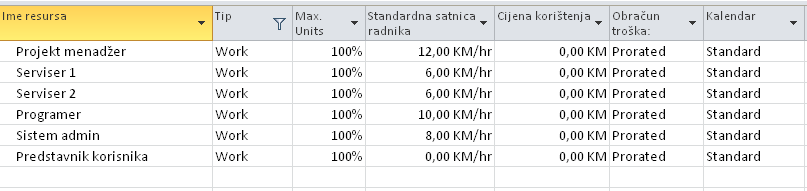
\includegraphics[width=15.5cm]{img/ljudski_resursi.png}
\caption{Pregled ljudskih resursa}
\end{table}

Raspored tima tokom realizacije projekta:

\begin{figure}[!h]
\centering
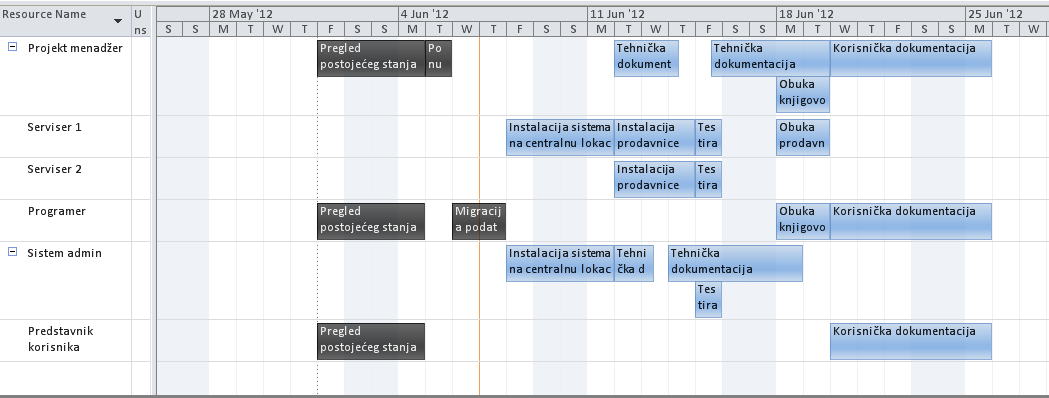
\includegraphics[width=15.5cm]{img/team_planner.png}
\caption{Pregled alokacije ljudskih resursa}
\end{figure}

Radi planiranja sastanaka uvršten je predstavnik klijenta. Zbog pravilne kalkulacije troškova sa stanovišta klijenta, troškovi predstavnika su 0 KM/h.

\pagebreak
\section{Finansijski aspekti}
\subsection{Budžet projekta}
\begin{table}[!h]
\centering
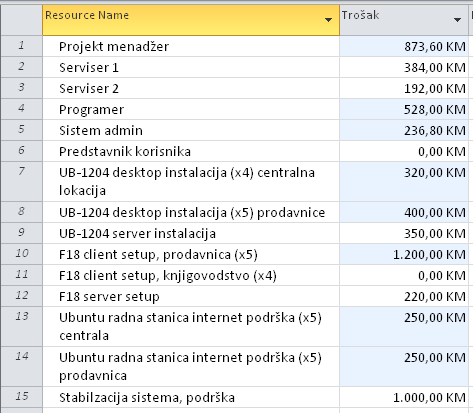
\includegraphics[height=7cm]{img/troskovi.png}
\caption{Pregled ukupnih troškova angažovanja resursa}
\end{table}

Ukupni troškovi realizacije projekta, uključujući fazu stabilizacije su \textbf{6204,40 KM}.

Navedeni su iznosi neto, bez uračunatog PDV-a.

\subsection{Finansiranje projekta}

Prodavac i klijent su dogovorili sjedeću dinamiku plaćanja:

\begin{table}[h]
\centering
\resizebox{15cm}{!} {
\begin{tabular}{ | r | c | c | r | }
\hline
Pozicija & preduslov za plaćanje & Vrijeme & Iznos (KM) bez PDV \\ \hline\hline
Avans: & - & 01.06.2012 & 2000 \\ \hline
Instalacija: & po okončanoj instalaciji & 01.07.2012 & 2000 \\ \hline
stabilizacija 1 & aktivna podrška klijentu & 01.08.2012 & 1000 \\ \hline 
stabilizacija 2 & aktivna podrška klijentu & 31.08.2012 & 1204.40 \\ \hline\hline 
                &                          &    UKUPNO: & 6204.40 \\ \hline
\end{tabular}
}
\caption{Dinamika plaćanja}
\end{table}

Ova dinamika omogućava klijentu da iz sopstvenih izvora (tekućih operativnih prihoda poslovanja \cite{prasorep}) finansira projekat.

\subsection{Ocjena opravdanosti investicije}

Analizu opravdanosti investicije bazirana je komparaciji sa alternativnimi rješenjem problema u kome korisnik jedino plaća troškove legalizacije postojećeg sistemskog sofvera.
Stoga u kalkulaciju nisu uzeti troškovi legalizacije uredskog "Microsoft office" software-a, niti nabavka novog ERP rješenja.

Kada bi se te stavke uvrstile u kalkulaciju opravdanosti, interna stopa rentabilnosti bi bila puno veća. Međutim, čak i u ovom konzervativnom scenariju troškova, naš projekat ima visoku internu stopu rentabilnosti od \textbf{36,9\%}, što nam sljedeća kalkulacija pokazuje:

\begin{table}[!h]
\centering
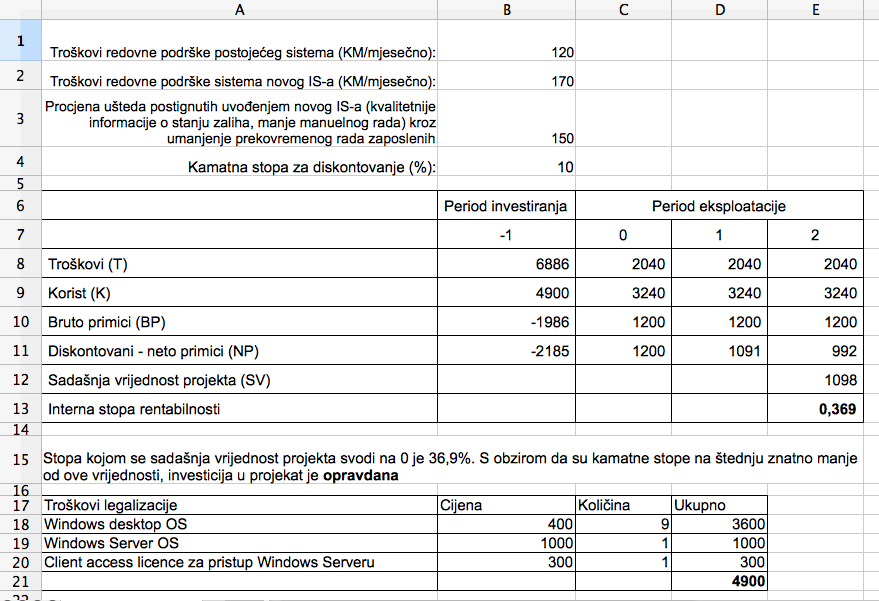
\includegraphics[height=10cm]{img/kalk_opravdanost.png}
\caption{Kalkulacija opravdanosti investicije}
\end{table}

\chapter{Zaključak}

Finansijski indikatori iz prethodnog poglavlja jasno kazuju da je predloženo IT rješenje u finansijskom smislu isplativa opcija. Troškovi licenci IS-a izgrađenog sa zatvorenim software-om \engl{proprietary software} su tako veliki, da će većina bosanskih poslovnih korisnika na licence potrošiti višegodišnji IT budžet. U tom slučaju budžetom se ne mogu predvidjeti sredstva za obuku, nadogradnju i kvalitetnu podršku IT sistemu. Smatramo će takvi korisnici, korisnici sa skromnim IT budžetom, u većini slučajeva dobiti bolji IS nabavkom otvorenog sistema. To vrijedi čak i u slučajevima kada su pojedinačne komponente zatvorenog IS-a superiorne u odnosu na otvoreni sistem.

Poslovni IT sistemi su složeni i dinamični sistemi. Ako korisnik nakon kupovine licenci ne može obezbjediti kvalitetnu obuku za osoblje i podršku, velika je vjerovatnoća da će konačnici dobiti sistem loših performansi, bez obzira što su pojedinačne komponente superiorne u odnosu na odgovarajući otvoreni sistem.

Na primjer, za najveći broj bosanskih poslovnih korisinika puno je bolje investirati u obuku za rad sa "LibreOffice"-om (LO) nego li kupovati licence za "Microsoft office" (MSO). Nakon kratke obuke, prosječan korisnik će sve poslove koje je obavljao sa MSO obavljati u LO istom brzinom i sa istim kvalitetom.

Naposlijetku, korištenje otvorenih sistema korisnicima otvara nove mogućnosti kod razvoja i nadogradnje IS-a.
Pored činjenice da je naš software iz primjera "LibreOffice" u poređenju sa "Microsoftovim" rješenjem dovoljno dobar \engl{good enough}, on ima jednu veoma bitnu prednost: "LibreOffice" je \textbf{multiplatformski} software. To znači da se LO može instalirati na različite platforme - različite operativnim sistema.

Multiplatformski software omogućava da se IS nadograđuje sa puno više slobode, što u finansijskom smislu redovno znači - puno jeftinije. Takva heterogena sistemska okruženja su s razlogom već postala standard u savremenim svjetskim IS-ovima.  

% -------------------------------------------------
\bibliography{literatura}
\bibliographystyle{fit}

% -------------------------------------------------
\appendix

\chapter{Korišteni software}
software korišten za realizaciju ovog dokumenta:
\begin{enumerate}
  \item Mac OS X 10.6.8
  \item Ubuntu Linux 12.04 Unity, 64bit
  \item mvim, vim tekst editor ver 7.3
  \item MacTex - pdfTeX 3.1415926-2.3-1.40.12 (TeX Live 2011)
  \item Windows XP Proffesional\footnote{kupac "bring.out" u sklopu MSDN Universal paketa, developer Ernad Husremović} on VirtualBox 4.1.16 MacOSX 
  \item Microsoft Project 2010, trial, ProductID 02252-552-2789414-37542
  \item LibreOffice 3.5.4
  \item Inkscape 0.4.8, Mac OSX X11
\end{enumerate}

\chapter{Bilješke}
\label{chap:biljeske}

\begin{itemize}
  \item izvorni kod dokumenta, \url{https://github.com/hernad/FIT_PRO/blob/master/latex/PRO_F18.tex}
  \item Dokumenta u PDF formatu, \url{https://github.com/hernad/FIT_PRO/raw/master/latex/PRO_F18.pdf}
  \item MS Project dokument \url{https://github.com/hernad/FIT_PRO/raw/master/F18_ubuntu_projekat.mpp}
  \item Calc dokument, kalkulacija opravdanosti investicije \url{https://github.com/hernad/FIT_PRO/raw/master/F18_ubuntu_projekat.ods}
\end{itemize}

\end{document}
